\chapter{Theory}
\paragraph{}
This section will discuss some important theory that is relevant to the literature and models discussed in Sections 3 and 4 respectively. The first part of the section briefly covers 2-degree of freedom vehicle dynamics and some of the existing control methods for autonomous vehicle control. The concept of model predictive control is then introduced, including the basic structure of an optimization problem involving MPC, its relevance to the control task of driving an autonomous vehicle, and a general framework for an MPC control system used in autonomous vehicles.

\section{A Brief Overview of Vehicle Dynamics}
\paragraph{}
This section discusses the kinematic and dynamic modeling of an autonomous car. A good vehicle model is essential for model-based control development, since the updates to the vehicle states rely on this model. 

\subsection{The Simple Kinematic Bicycle Model}
\begin{figure}[H]\label{fig2.1}
\centering 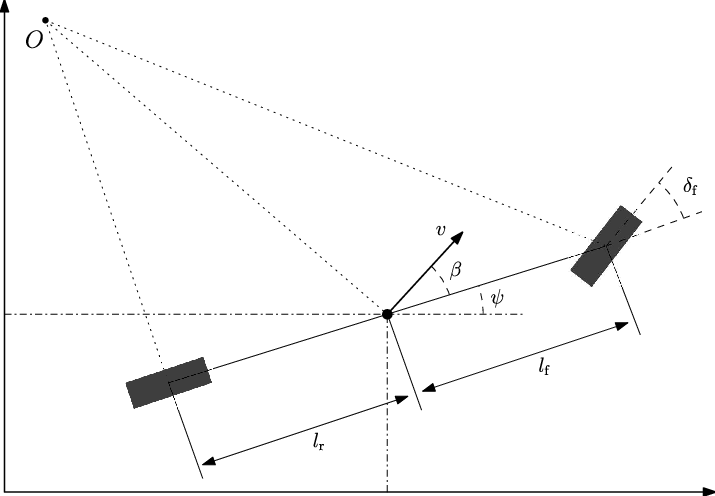
\includegraphics[scale = 0.45]{Images/simple_bicycle_model.png}
\caption{The Simple 2-DOF Bicycle Model}
\end{figure}

\paragraph{}
In most self driving control problems, the vehicle is modelled after the 2-DOF bicycle model. This is a classic kinematics model that does surprisingly well at capturing vehicle motion in normal driving conditions. This also eliminates the computational difficulties associated with other models that attempt to model the equations of each wheel separately, resulting in a highly non-linear vehicle model. Figure 2.1 illustrates the simple bicycle model with the reference point at the center of gravity. Similar models can be developed with front \& rear wheel references.

\paragraph{}
The model accepts the velocity $v$ and the rate of change of the steering angle $\varphi$ as inputs. The angle $\psi$ is known as the vehicle heading or the yaw angle. The bicycle kinematics are governed by the following set of equations:
$$\begin{array}{r}
    \text{Inputs: }\begin{bmatrix}[1] v & \varphi\\ \end{bmatrix}^T\\
    \text{States: }\begin{bmatrix}[1] x & y & \theta & \delta\\ \end{bmatrix}^T
\end{array}\longrightarrow\left\lbrace\begin{array}{l}
    \dot{x_c} = v\cos(\psi + \beta),\text{ } \dot{y_c} = v\sin(\psi + \beta)\\
    \dot{\psi} = \dfrac{v\cos\beta\tan\delta_f}{l_r+l_f},\text{ } \dot{\delta_f} = \omega\\
    \dot{\beta} = \tan^{-1}\left(\dfrac{l_r\tan\delta_f}{l_r + l_f}\right)
\end{array}\right.$$

\subsection{Modeling Vehicle States}
When dealing with vehicle states, we generally express the equations of motion in the state-space form, as follows:
$$\begin{Bmatrix}[1] \dot{x}\\ y \end{Bmatrix} = \begin{bmatrix}[1] A & B\\ C & D \end{bmatrix}\begin{Bmatrix}[1] x\\ u \end{Bmatrix}$$

\paragraph{}
The vectors $x$, $y$ and $u$ represent the states of the system, while the $A$, $B$, $C$ and $D$ matrices represent the system, input, output and feed-through respectively. The matrices for a continuous-time vehicle model are defined as follows:
$$A = \begin{bmatrix}[1]
    0 & 0 & -v\sin\psi & \cos\psi\\
    0 & 0 & v\cos\psi & \sin\psi\\
    0 & 0 & 0 & \dfrac{\tan\delta}{L_c}\\
    0 & 0 & 0 & 0
\end{bmatrix}\hspace{1cm}
B = \begin{bmatrix}[1]
    0 & 0\\
    0 & 0\\
    0 & \dfrac{v(\tan^2\delta + 1)}{L_c}\\
    0.5 & 0
\end{bmatrix}$$
where $L_c$ denotes the length of the car's wheelbase (i.e., distance from the centers of the rear wheel to the front wheel). The remaining matrices are usually defined as $C = \begin{bmatrix}[1]
    \text{I} & 0
\end{bmatrix}$, and $D = 0$. In instances of linear MPC control problems, the continuous-time model is converted into a linear model by discretizing the matrices $A$ and $B$.

\subsection{Modeling Vehicle Dynamics using Tire Parameters}
\paragraph{}
Dynamic modeling of a vehicle is more computationally complex compares to kinematic modeling, since it takes into account forces and torques acting on the vehicle. However, a dynamic model can lead to higher fidelity predictions that are not possible with kinematic models. Also, kinematic models implicitly assume a no-slip condition that is followed by the vehicle. However, at high speeds or on slippery road surfaces, this condition is not satisfied. In such cases, the throttle and steering inputs are governed by forces such as drag and friction. 

\paragraph{}
Tire modeling has been extensively researched, and there are highly non-linear models such as the Pacejka and Dugoff tire models that accurately dictate the rotational dynamics of a vehicle. In this section, however, we limit ourselves to a simpler vehicle model which uses the bicycle model discussed earlier, which is shown in Figure 2.2.

\begin{figure}[H]\label{fig2.2}
\centering 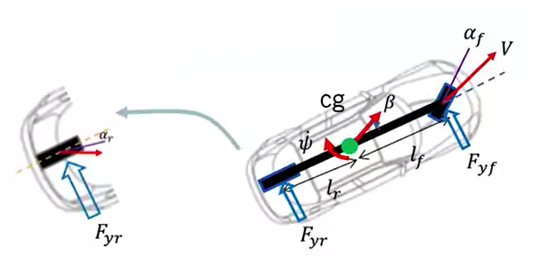
\includegraphics[scale = 1.2]{Images/vehicle_dynamics_model.png}
\caption{A Simple Vehicle Dynamics Model}
\end{figure}
\paragraph{}
The total acceleration in the inertial frame is defined as $a_y = \ddot{y}+\omega^2R=V\dot{\beta}+V\dot{\psi}$, which includes the lateral acceleration in the body frame and the centripetal acceleration. The angles $\beta$ and $\psi$ are defined as the slip angle and vehicle heading respectively. Since the only two forces affecting the lateral dynamics of the vehicle are $F_{yr}$ and $F_{yf}$, the model can now be formulated as:
\begin{align*}
    mV(\dot{\beta}+\dot{\psi})&=F_{yf}+F_{yr}\\
    I_z\ddot{\psi}&=l_fF_{yf}-l_rF_{yr}
\end{align*}
where $I_z$ denotes the vehicle's inertia about an axis perpendicular to the plane of the vehicle and passing through its center of gravity. For modeling the tire dynamics, we then introduce a linear tire model based on its front and rear tire slip angles. We define the cornering stiffness of the two wheels $C_f$ and $C_r$ as the ability of the wheels to resist deformation as the vehicle corners (i.e., the ratio of lateral force on the wheel to the tire slip angle). By modifying the above equations accordinaly, we obtain the following equations for the $A$ and $B$ matrices for the vehicle dynamics model:
$$\left.\begin{array}{r}
    \text{States: } \begin{bmatrix}[1] y & \beta & \psi & \dot{\psi}\end{bmatrix}^T\\
    \dot{X_{lateral}}=A_{lat}X_{lateral} + B_{lat}\delta 
\end{array}\right\rbrace\longrightarrow
A = \begin{bmatrix}[1]
    0 & V & V & 0\\
    0 & -\dfrac{C_r + C_f}{mV} & 0 & \dfrac{C_rl_r - C_fl_f}{mV^2} - 1\\
    0 & 0 & 0 & 1\\
    0 & \dfrac{C_rl_r - C_fl_f}{I_z} & 0 & -\dfrac{C_rl_r^2 + C_fl_f^2}{I_zV} - 1
\end{bmatrix}\hspace{5mm}
B = \begin{bmatrix}[1]
    0\\ \dfrac{C_f}{mV}\\ 0\\ \dfrac{C_fl_f}{I_z}
\end{bmatrix}$$

\section{Existing Methods for Control of Self-Driving Vehicles}
\paragraph{}
This section discusses the basic concepts regarding some existing longitudinal and lateral control techniques to control the speed of the vehicle and its steering output respectively.

\subsection{Proportional-Integral-Derivative Control}
\paragraph{}
One of the most widely used control techniques for longitudinal control of a vehicle is proportional-integral-derivative (PID) control. PID control is mathematically formulated by adding three terms dependent on the error function of the system. As the names suggest, the proportional term is directly proportional to the error $e(t)$, the integral term is proportional to the integral $\displaystyle\int_0^te(t)\text{d}t$, and the derivative term is proportional to its derivative $\dot{e}(t)$. The response of the PID controller in the time domain is expressed as follows:
$$u(t)=K_Pe(t)+K_I\int_0^te(t)\text{d}t+K_D\dot{e}(t)$$
where $K_P$, $K_I$ and $K_D$ represent the proportional, integral and derivative gains respectively. The PID control loop is illustrated in Figure 2.3.

\begin{figure}[H]\label{fig2.3}
\centering 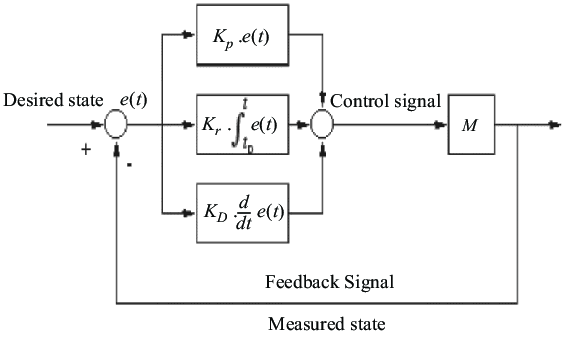
\includegraphics[scale = 0.5]{Images/pid_control_system.png}
\caption{Feedback Loop for a PID Control System}
\end{figure}

\noindent Taking the Laplace transform of the PID control equation yields the following response in the frequency domain:
\begin{align*}
    U(s) = G(s)E(s) &= \left(K_P + \dfrac{K_I}{s}+ K_Ds\right)E(s)\\
    &= \left(\dfrac{K_Ds^2 + K_Ps + K_I}{s}\right)E(s)
\end{align*}

\paragraph{}
The transfer function has only one pole at the origin, and the zeroes are located arbitrarily on the complex plane. Therefore, PID control design boils down to achieving the desired output response selecting zero locations by selecting PID gains. There are several algorithms for tuning PID gains, which will not be discussed in the report. Note that not all gains need to be used for all control systems. One or more of the controller gains can be set to zero to obtain a P, PD or PI control system.

\paragraph{}
In the context of autonomous vehicle control, PID controllers are employed for the task of cruise control. ACC systems usually employ a high level and low level controller. The high level controller is a PID controller, while the low level controller generates the throttle/brake outputs depending on the PID controller response. To maintain a desired velocity, the PID control system is set up as follows:
$$\ddot{x_{des}} = K_P(\dot{x_{ref}} - \dot{x}) + K_I\int_0^t(\dot{x_{ref}} - \dot{x})\text{d}t + K_D\dfrac{\text{d}(\dot{x_{ref}} - \dot{x})}{\text{d}t}$$

\subsection{Pure Pursuit Control}
\paragraph{}
Pure pursuit control (PPC) is a geometric path tracking control strategy used for lateral steering control. The control objective is to compute the front wheel angle $\delta$ such that the vehicle follows a given path. In the PPC method, a target point on the desired path is identified, which is a look-ahead distance $l_d$ away from the vehicle's current position. The angle $\delta$ is chosen such that the vehicle will reach the target point according to the kinematic bicycle model. Figure 2.4 illustrates the geometric aspects of PPC design.

\begin{figure}[H]\label{fig2.4}
\centering 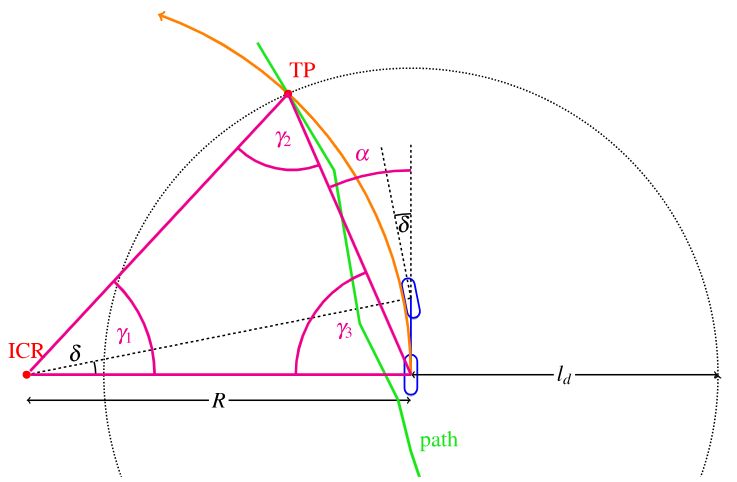
\includegraphics[scale = 0.7]{Images/ppc_diagram.png}
\caption{Geometric Aspects of Pure Pursuit Control Design}
\end{figure}
\paragraph{}
Note that the triangle formed by the instantaneous center of rotation, the target point and the vehicle's rear wheel is isosceles, which results in $\gamma_2 = \gamma_3 = 90\degree - \alpha$ and $\gamma_1 = 2\alpha$. Using the law of sines, we get the following relation between $R$ and $l_d$:
$$\frac{l_d}{\sin\gamma_1} = \frac{R}{\sin\gamma_2}\implies\frac{l_d}{\sin2\alpha} = \frac{R}{\cos\alpha}\implies l_d = 2R\sin\alpha$$

\noindent This yields the final steering output as ($L$ is the distance between the rear and front wheel centers): $$\delta=\tan^{-1}\left(\frac{2L\sin\alpha}{l_d}\right)$$

\paragraph{}
Note that the reponse of a pure pursuit controller is independent of the vehicle speed. This is ideal for ease of computations, but is likely to result in sluggish responses at high speeds and aggressive responses at very low speeds. To remedy this, the inclusion of a pure pursuit gain is proposed.
$$l_d = K_{pp}V\implies \delta=\tan^{-1}\left(\frac{2L\sin\alpha}{K_{pp}V}\right)$$

\subsection{The Stanley Controller}
\paragraph{}
The Stanley controller is another control technique used for lateral steering control of a vehicle. This controller was devised and used by the Stanford racing team in the second DARPA grand challenge. The Stanley controller makes use of the center of the front axle as the reference point, and looks at both the heading and the positional errors relative to the closest point on the path. Figure 2.5 illustrates the geometric details of the Stanley control problem.
\begin{figure}[H]\label{fig2.5}
\centering 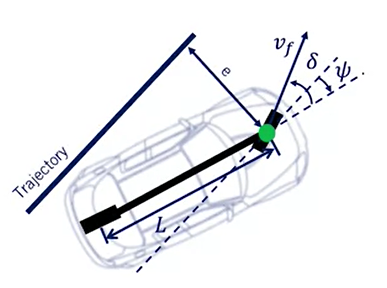
\includegraphics[scale = 1]{Images/stanley_controller.png}
\caption{Geometric Design Aspects of the Stanley Controller}
\end{figure}

\paragraph{}
The Stanley controller has three main components, which are detailed as follows:
\vspace{-2.5mm}

\begin{enumerate}[label=(\arabic*), itemsep=0em]
    \item Adjust the steering angle to align the vehicle's heading with the desired heading, i.e., $\delta(t) = \psi(t)$
    \item A proportional control is added to eliminate the cross-track error $e(t)$, whose gain is determined experimentally. The updated equation for the steering angle is: $$\delta(t) = \psi(t) + \tan^{-1}\left(\frac{ke(t)}{v_f(t)}\right)$$
    \item the steering angle must stay within the maximum and minimum bounds, i.e., $\delta\in[\delta_{min},\delta_{max}]$
\end{enumerate}

\paragraph{}
The steering angle is adjusted according to the relative magnitude of the heading and cross-track errors. The Stanley controller suffers from the same difficulty as PPC when faced with low speeds. In order to avoid an aggressive steering response, a softening constant $k_s$ is added to the control law:
$$\delta(t) = \psi(t) + \tan^{-1}\left(\frac{ke(t)}{k_s+v_f(t)}\right)$$

\section{Introduction to Model Predictive Control}
\paragraph{}
Model Predictive Control is a discrete-time multi-variable control architecture. MPC uses the current plant measurements, the current dynamic state of the process, the MPC models, and the process target variables and limits to compute the future changes in the system's dependent variables. As discussed earlier in Section 1, MPC has seen wide applications in advanced process control in chemical industries. The use of MPC is relatively new in the autonomous driving industry, and significant amount of research is being carried out to make MPC models, especially non-linear ones, implementable in real-time.

\paragraph{}
MPC is based on iterative, finite-time horizon optimization of a plant model. At time $t$, the current plant state is sampled and a cost minimizing control prediction is computed for a relatively short time horizon $[t, t+T]$. This is known as the prediction horizon. A numerical minimization algorithm is used to compute the optimal control strategies for all the time intervals starting from the current time up to the prediction horizon. 

\paragraph{}
The control horizon, on the other hand, is the section of the prediction horizon in which control moves are allowed. This is different from the prediction horizon, in that the optimal control strategy is only computed across the prediction horizon, while the control inputs are actually manipulated in the control horizon. A general rule of thumb is to set the control horizon to around 10-20\% of the prediction horizon.

\paragraph{}
Once the optimal control strategies have been computed by the optimization algorithm, the MPC controller implements only the first control strategy. The plant state is then sampled again and the calculations described above are repeated for the new current state, yielding a new set of optimal control strategies and new predicted state path. The prediction horizon keeps shifting forward as the MPC algorithm proceeds, which makes MPC an example of receding horizon control. Figure 2.6 illustrates a basic MPC control loop. 
\begin{figure}[H]\label{fig2.5}
\centering 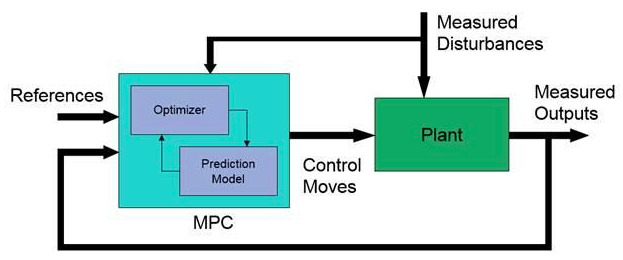
\includegraphics[scale = 0.6]{Images/mpc_control_loop.png}
\caption{Basic MPC Control Loop}
\end{figure}

\paragraph{}
Model predictive control is, hence, a multi-variable control algorithm that uses an internal dynamic model of the process, a cost function $J$ over the receding horizon, and an optimization algorithm minimizing the cost function $J$ using the control input $u$. An example of a quadratic cost function for the MPC optimization problem is given by:
$$J=\sum_{i=1}^Nw_{x_i}(r_i-x_i)^2+\sum_{i=1}^Mw_{u_i}\Delta u_i^2$$
\vspace{-12.5mm}

\begin{align*}
    \text{where }\text{ }\text{ }\text{ }x_i&: i^{\text{th}}\text{ controlled variable}\hspace{0.7\textwidth}\\
    r_i&: i^{\text{th}}\text{ reference variable}\hfill\\
    u_i&: i^{\text{th}}\text{ manipulated variable/control input}\hfill\\
    w_{x_i}&:\text{weighting coefficient reflecting the relative importance of }x_i\hfill\\
    w_{u_i}&:\text{weighting coefficient penalizing relative big changes in } u_i\hfill
\end{align*}

\paragraph{}
LQR is another optimal control method that has a quadratic cost function. While MPC looks at weighted sets of error functions, the LQR algorithm looks at all linear system inputs and computes a transfer function that minimizes the total error. Further, LQR optimizes over the entire time window and the same solution is often employed for the entire operating time, while MPC optimizes over a receding time horizon. Due to these fundamental differences, MPC is likely to obtain sub-optimal solutions for some time steps. However, since MPC makes no assumptions about linearity of system inputs, it can handle hard constraints. This difference is discussed in greater detail in section 3.2.

\subsection{General MPC Framework for Self-Driving Vehicles}
\paragraph{}
Model predictive control can be employed in several autonomous driving applications, both for lateral as well as longitudinal control, to improve vehicle responsiveness while maintaining passenger safety and comfort. Some features of MPC that are useful for autonomous driving are:
\vspace{-2.5mm}

\begin{itemize}[itemsep=0em]
    \item MPC can explicitly handle input and output constraints, which makes it very easy to impose limits on speed \& acceleration limits, safe following distance, steering angle \& steering rate limits, and constraints regarding obstacles in the vicinity of the vehicle
    \item MPC uses an internal model of vehicle dynamics to predict the behaviour of the ego vehicle across a receding time horizon. This enables the system to preview reference trajectories and disturbances over the prediction horizon.
    \item Adaptive MPC allows updating of the internal vehicle model at run time. This is especially useful in cases where the dynamics of the ego vehicle vary with time, such as for velocity-dependant steering dynamics. 
\end{itemize}

\paragraph{}
MPC also deals with several drawbacks of classical control systems. Firstly, it integrates the lateral and longitudinal control instead of treating them as separate aspects of the self-driving task. It also does not require any tuning of controller gains, which may be a difficulty in traditional control systems making use of several PID controllers along with Stanley/PPC controllers. Finally, it can handle constraints on control inputs, vehicle states and obstacles directly as part of the optimization problem instead of employing a separate system that deals with environmental input from image sensors on the car.

\paragraph{}
A common driving task where MPC is employed is path tracking and obstacle avoidance. The following optimization problem setup can be used for the above driving scenarios:
\begin{align*}
    \min_{x_{1:T}, u_{1:T}} & J(x_{1:T}, u_{1:T}) = \sum_{t=1}^T e^{\prime}Qe + u^{\prime}Ru\\
    \text{s. t. }\text{ }\text{ } & x_{t+1} = f(x_t, u_t)\hspace{31.5mm}\forall t\in[1, T-1]\\
    & \dot{x}_t\in[\dot{x}_{min}, \dot{x}_{max}]\hspace{32mm}\forall t\in[1, T]\\
    & u_t\in[u_{min}, u_{max}],\text{ }\dot{u}_t\in[\dot{u}_{min}, \dot{u}_{max}]\hspace{5mm}\forall t\in[1, T]\\
    & u_t\in\mathcal{U}_t,\text{ }x_t\in\mathcal{X}_t\hspace{30mm}\forall t\in[1, T]\\
    & \text{(obstacle \& other constraints)}
\end{align*}

\noindent where $e=\abs{x_{ref}-x}$ represents the error in reference tracking, $Q$ and $R$ represent the weighting matrices for the trajectory error and vehicle inputs respectively, and $\mathcal{X}_t$ \& $\mathcal{U}_t$ represent the range space of the vehicle states and inputs respectively. $\mathcal{X}_t$ and $\mathcal{U}_t$ together are often referred to as the vehicle's operational design domain (ODD).

\paragraph{}
Of course, this list of constraints is not exhaustive, and more constraints can be added as necessary. For example, certain driving applications might necessitate constraints on the vehicle's acceleration. The vehicle might also encounter obstacles only after a certain time has passed, in which case, the constraints have to be dynamically added to the model. The use of MPC for various driving applications is illustrated in Section 4.
